\documentclass[12pt,twocolumn]{article}
\usepackage{lmodern,setspace,amsmath,amssymb,amsfonts,amsthm,graphicx,multicol}
\usepackage[a4paper, top=0.9in, bottom=1.15in]{geometry}
\usepackage[polish]{babel}
\usepackage[utf8]{inputenc}
\title{Algorytmy i struktury danych - Programowanie dynamiczne}
\author{Dariusz Max Adamski}
\date{}

\begin{document}

\maketitle


\section*{Wstęp}

W tym sprawozdaniu będzie porównywana efektywność algorytmu zachłannego,
przeszukiwania wyczerpującego oraz algorytmu dynamicznego,
w rozwiązywaniu problemu plecakowego.
Skonfrontowane będą także algorytmy pod względem jakości uzyskanych rozwiązań.


\section{Metodologia}

Czasy dla przeszukiwania wyczerpującego ,,BF'' były mierzone na $n = 14..28$.
Dla algorytmu dynamicznego ,,DP'' oraz zachłannego ,,GA'' zostały także badane instancje o 
$n$ od $100$ do $2\ 000$ co $100$.
Parametr $b$ jest niezależny od $n$, był wybierany losowo z przedziału $[10\ 000, 1\ 000\ 000]$.
Przedmioty miały losowo dobieraną wagę $w$ z przedziału $[10, 1000]$, a wartość $v$ z przedziału $[100, 10\ 000]$.
Parametr $y$ jest obliczany ze wzoru $y = \beta \cdot \sum_{i=1}^n v_i$, gdzie $\beta \in (0, 1]$.

Do wykonania wykresu 3D mierzono czas ,,DP'' dla każdej pary $\langle n, b \rangle$ z iloczynu kartezjańskiego $N \times B$, gdzie
$N = B = \{10, 50, 100, 500, 1000, 2000, 5000, 10000, \\ 15000, 20000, 25000, 30000\}$.
Instancje wybrane do mierzenia jakości rozwiązań są opisane w sekcji ,,Jakość rozwiązań''

Optymalizacje kompilatora zostały wyłączone flagą ,,-O0''. 
Czas wykonywania był mierzony w nanosekundach.

\section{Efektywność algorytmów}

\begin{figure}[h]
	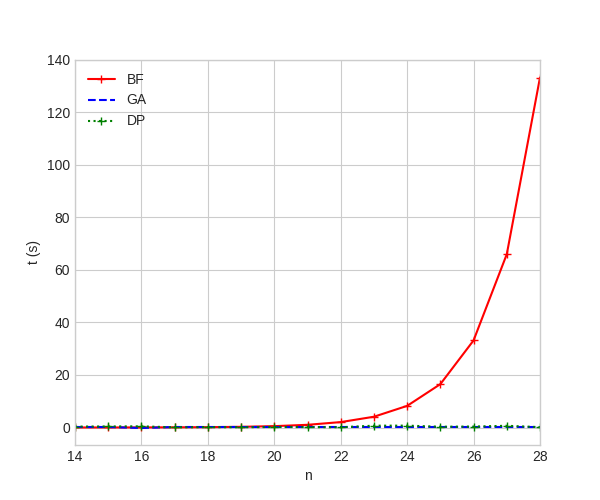
\includegraphics[width=\linewidth]{speed-n.png}
	\caption{Efektywność algorytmów w zależności od $n$ \label{speed_n}}
\end{figure}

\begin{figure}[h]
	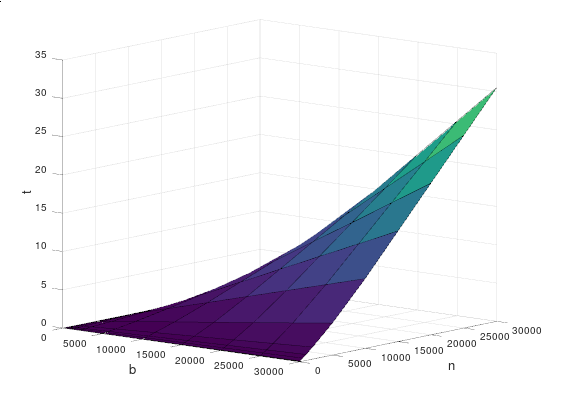
\includegraphics[width=\linewidth]{speed-bn.png}
	\caption{Efektywność DP w zależności od $n$ i $b$ \label{speed_bn}}
\end{figure}

Algorytm BF ma złożoność $O(2^n)$, co widać na wykresie \ref{speed_n}.
Krzywa BF może być aproksymowana przez funkcję
$BF'(n) = 2^n \cdot C \approx 2^{n - 20.6}$.

\begin{figure}[h]
	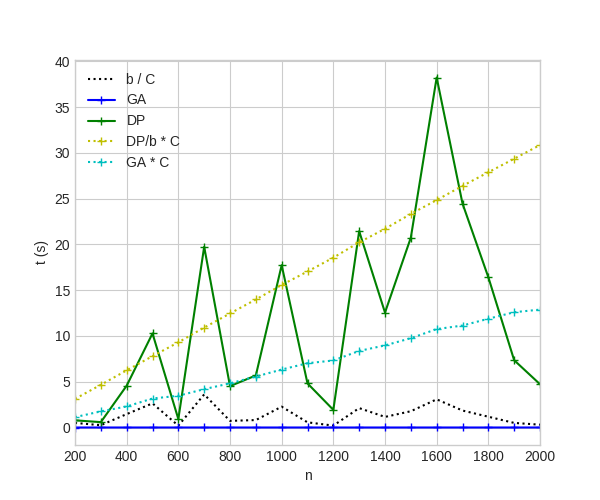
\includegraphics[width=\linewidth]{speed-n-big.png}
	\caption{Efektywność algorytmów w zależności od $n$ \label{speed_n_big}}
\end{figure}


Czasy wykonywania GA oraz DP dla $n > 28$, są przedstawione na wykresie \ref{speed_n_big}.
Złożoność GA jest zależna od złożoności obliczeniowej zastosowanego algorytmu sortującego,
tutaj $O(n \log n)$ w każdym przypadku. Rzeczywisty czas wykonywania jest oznaczony jako GA.
Funkcja została także przeskalowana o stałą $C$ i przedstawiona na wykresie jako ,,GA * C'',
aby lepiej zilustrować czas wykonywania.

Analiza złożoności DP jest trudniejsza, 
ponieważ zależy ona od dwóch zmiennych $b$ oraz $n$.
Na wykresie \ref{speed_n_big} jest przedstawiona funkcja $DP/b$,
przeskalowana o stałą $C$ która pokazuje, że 
DP rośnie liniowo w zależności od $n$.

\begin{figure}[h]
	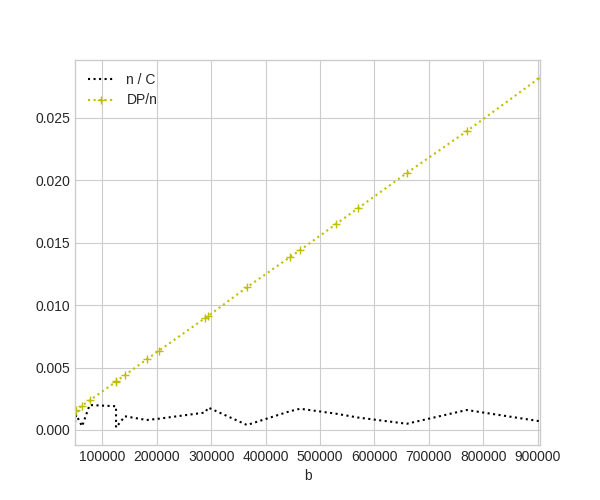
\includegraphics[width=\linewidth]{speed-b-big.png}
	\caption{Efektywność algorytmów w zależności od $b$ \label{speed_b_big}}
\end{figure}

Następnie na wykresie \ref{speed_b_big} została przedstawiona zależność ,,DP/n'' 
Jak widać DP rośnie także liniowo w zależności od $b$.
Dodatkowo na wykresie znajduje się relacja $n$ od $b$, przeskalowana o stałą $C$.
Natomiast rysunku \ref{speed_bn} została pokazana efektywność DP w zależności od $b$ oraz $n$.

Aby mieć pewność, że $b$ nie jest zależne od $n$, na rysunku \ref{speed_n_big} została
pokazana relacja $b$ od $n$, przeskalowana o stałą $C$.
Jak widać, jest ona losowa.
Możemy więc potwierdzić, że złożoność DP to faktycznie $O(b \cdot n)$.


Ewentualne odchylenia są spowodowane losowością instancji problemu.


\section{Jakość rozwiązań}

\begin{figure}[h]
	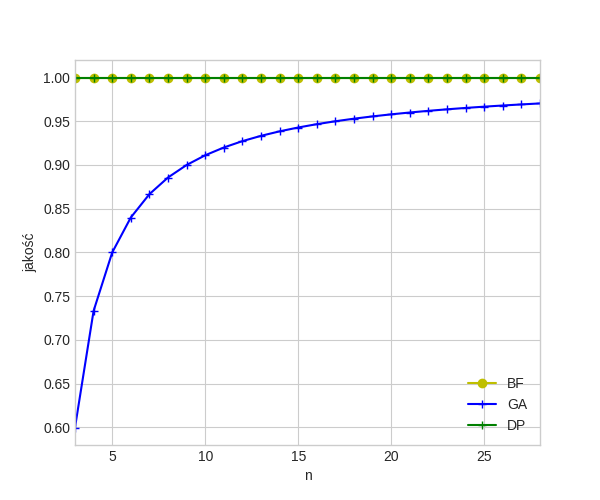
\includegraphics[width=\linewidth]{quality.png}
	\caption{Jakość rozwiązań od $n$ \label{quality}}
\end{figure}

Algorytm GA nie rozwiązuje problemu plecakowego, a jedynie przybliża jego rozwiązanie.
Na rysunku \ref{quality} widać, że jakość rozwiązań GA jest mniejsza od DP oraz BF,
przy czym zaznaczając, że te metody rozwiązują problem plecakowy.

\begin{figure}[h]
	$$b \leftarrow 20,\ y \leftarrow 10$$
	\begin{center}
		\begin{tabular}{|l|r|r|r|}
			\hline
			$v$ & 6 & 5 & 5 \\ \hline
			$w$ & 11 & 10 & 10 \\ \hline
		\end{tabular}
	\end{center}
	\caption{Problematyczna instancja \label{evil}}
\end{figure}

Aby zmierzyć jakość aproksymacji rozwiązania przez GA, wygenerowane zostały specjalne
instancje problemu, które mają na celu działanie na szkodę wybranej heurystyki.
W tych instancjach wszystkie przedmioty mają $v = 5$ oraz $w = 10$, ale jeden przedmiot ma $v/w > 0.5$
Przykładowa instancja tego typu jest przedstawiona w tabelce \ref{evil}.

Zastosowana heurystyka sprawia, że specjalny element zostanie wybrany, a na resztę zabraknie miejsca.


\section{Klasa problemu}

\begin{figure}
	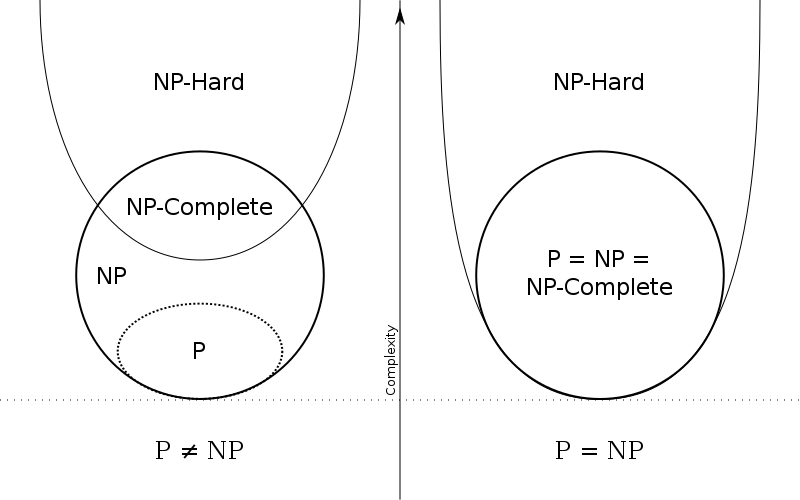
\includegraphics[width=\linewidth]{pnp.png}
	\caption{Diagram klas problemów \label{pnp}}
\end{figure}

Problem plecakowy jest problemem należącym do części wspólnej klas NP oraz NP-hard, czyli NP-complete,
zakładając że $P \neq NP$ (rysunek \ref{pnp}).
Oznacza to, że operacja znajdywania rozwiązania problemu ma złożoność najwyżej wykładniczą.
Możemy jednak zweryfikować znalezione rozwiązanie w czasie wielomianowym.


\section{Podsumowanie}

Podsumowując, metodą najlepiej rozwiązującą problem plecakowy
jest programowanie dynamiczne. Ta metoda działa zdecydowanie szybciej od
przeszukiwania wyczerpującego i w odróżnieniu od algorytmu zachłannego
nie aproksymuje rozwiązania.
Jednak jeżeli możemy pozwolić sobie na przybliżenie rozwiązania,
algorytm zachłanny zapewnia je w czasie wielomianowym.

\end{document}
